% Created 2024-06-22 Sat 21:04
% Intended LaTeX compiler: pdflatex
\documentclass[11pt]{article}
\usepackage[utf8]{inputenc}
\usepackage[T1]{fontenc}
\usepackage{graphicx}
\usepackage{longtable}
\usepackage{wrapfig}
\usepackage{rotating}
\usepackage[normalem]{ulem}
\usepackage{amsmath}
\usepackage{amssymb}
\usepackage{capt-of}
\usepackage{hyperref}
\usepackage[a4paper,left=1cm,right=1cm,top=1cm,bottom=1cm]{geometry}
\usepackage[american]{babel}
\usepackage{enumitem}
\usepackage{float}
\usepackage[sc]{mathpazo}
\linespread{1.05}
\renewcommand{\labelitemi}{$\rhd$}
\setlength\parindent{0pt}
\setlist[itemize]{leftmargin=*}
\setlist{nosep}
\author{Marcio Woitek}
\date{}
\title{TSP Integer Programming}
\hypersetup{
 pdfauthor={Marcio Woitek},
 pdftitle={TSP Integer Programming},
 pdfkeywords={},
 pdfsubject={},
 pdfcreator={Emacs 29.3 (Org mode 9.6.24)}, 
 pdflang={English}}
\begin{document}

\maketitle
\thispagestyle{empty}
\pagestyle{empty}

All problems are related to the graph below. Black edges have weight 1, and red
edges have weight 2.
\begin{figure}[H]
  \centering
  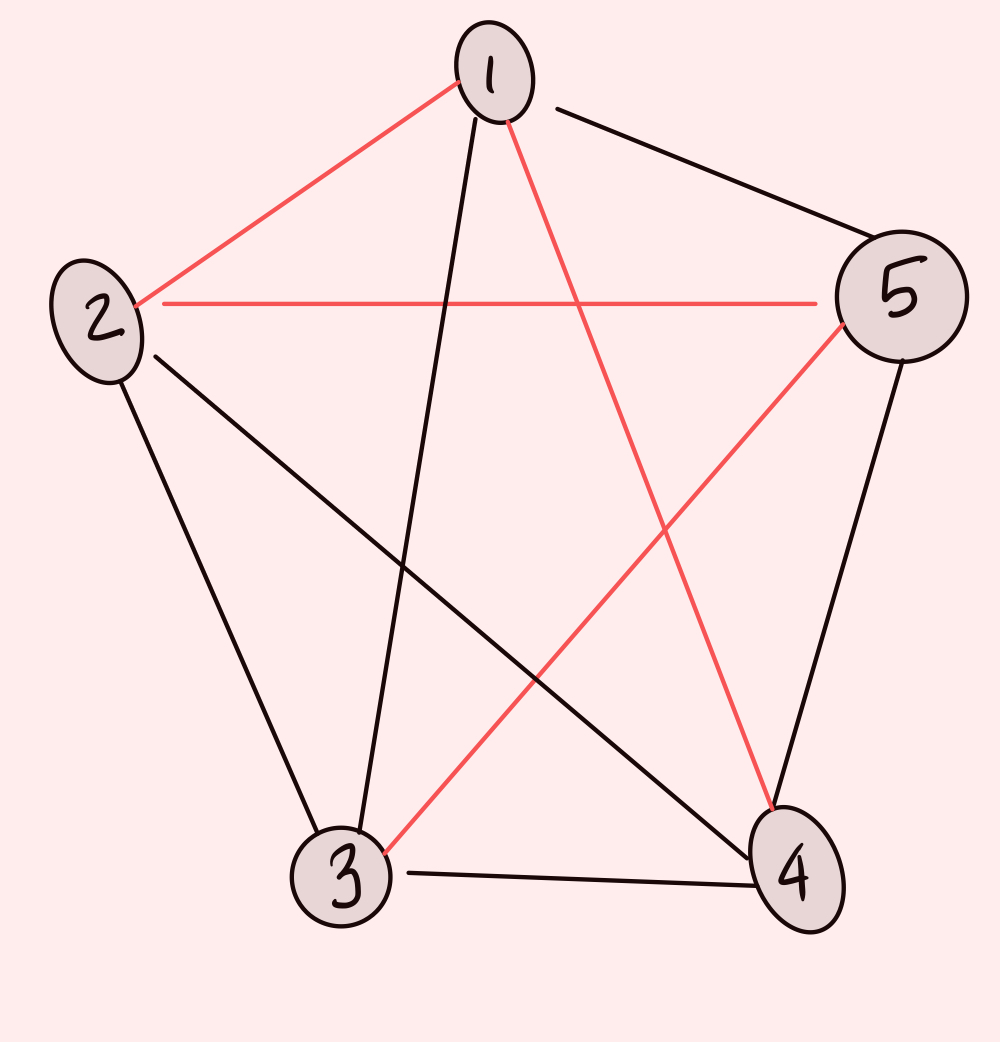
\includegraphics[scale=0.15]{held_karp_graph.jpeg}
  \caption{TSP instance}
\end{figure}

\section*{Problem 1}
\label{sec:orgb2611d7}
\begin{itemize}
\item Setting the variable \(x_{i,j}=1\) denotes that we go from vertex \(i\) to
\(j\) using the edge \((i,j)\) in our tour.
\item The constraint \(x_{2,1}+x_{3,1}+x_{4,1}+x_{5,1}=1\) expresses that we have
exactly one edge entering the vertex 1 in our tour.
\end{itemize}

\section*{Problem 2}
\label{sec:orgca4dc97}
\begin{itemize}
\item Time stamp variables \(t_2\), \(t_3\), \(t_4\), \(t_5\) are added to eliminate
possible subtours by assigning increasing time stamps to nodes visited along a
tour.
\item The constraint \(t_3\geq t_2+x_{2,3}-M(1-x_{2,3})\) for a large number \(M\)
is equivalent to if \((x_{2,3}=1)\) then \(t_3\geq t_2+1\) else \(t_3\geq t_2-M\).
\end{itemize}

\section*{Problem 3}
\label{sec:orgd30e8f3}
\begin{itemize}
\item \(x_{2,4}+x_{3,4}+x_{5,4}+x_{2,1}+x_{3,1}+x_{5,1}\geq 1\)
\item \(x_{4,2}+x_{4,3}+x_{4,5}+x_{1,2}+x_{1,3}+x_{1,5}\geq 1\)
\end{itemize}
\end{document}
